\newpage


\section{Введение}
\label{submission}

В последние годы SOTA \cite{yu2023noisynn}-подходы к классификации изображений достигли значительных показателей точности. Основным бенчмарком для проверки качества таких моделей является ImageNet LSVRC \cite{russakovsky2015imagenet}, а наиболее продвинутые модели обучаются от нескольких недель до месяцев на таких масштабных датасетах, как JFT-300M \cite{sun2017revisiting} и ImageNet-21K \cite{5206848} на множестве GPU-машин. Хотя классические современные решения, такие как ViT \cite{dosovitskiy2021image} и другие модели Vision Transformer, превосходят решения на основе ResNet \cite{he2015deep}, хотя для предварительного обучения требуется значительно меньше вычислительных ресурсов, они по-прежнему работают как черный ящик. Получив на вход мини-пакет изображений и необходимые метки, они выдают готовое распределение по меткам классов. В этом случае целью подхода Concept Bottleneck Models \cite{koh2020concept} является разработка моделей, которые бы отвечали на такие вопросы, как: "Почему вы выбрали именно этот класс?", "На основании каких результатов вы его предсказали?". Предполагается, что этот подход будет чрезвычайно полезен в областях, где объяснения имеют решающее значение, например в медицинских приложениях. 

\begin{figure}[t]
\begin{center}
\centerline{
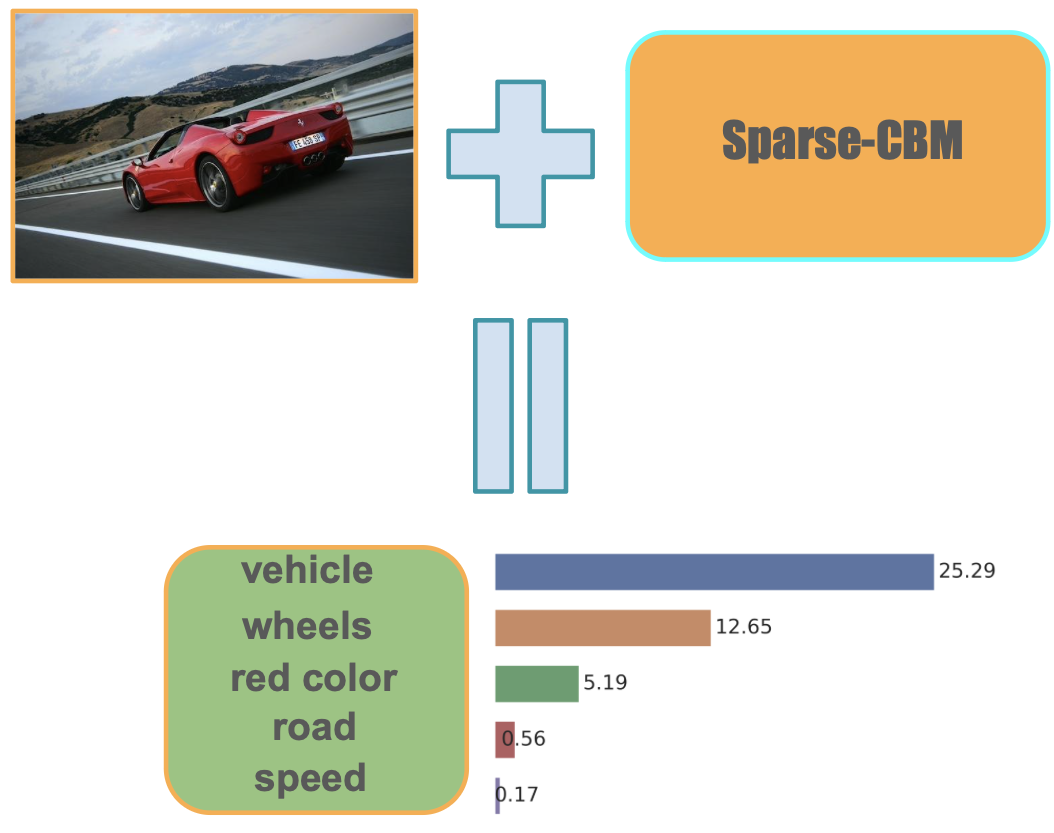
\includegraphics[width=0.55\columnwidth]{./figures/opening_test_3.png}}
\caption{Пример концептов, отобранных Sparse-CBM.}
\label{fig:opening}
\end{center}
\vskip -0.4in
\end{figure}
Мы изучаем модели, которые сначала предсказывают промежуточный набор понятных человеку понятий, а затем используют его для предсказания конечной метки, поддерживаемой выбранными понятиями. Построение интерпретируемых нейронных сетей стало более популярным с представлением модели OpenAI CLIP \cite{radford2021learning} и развитием методов контрастивного обучения \cite{aljundi2022contrastive}. Нельзя не отметить растущее направление мультимодальности \cite{reed2022generalist,chen2023sharegpt4v} с его многообещающими результатами по объединению нескольких модальностей, таких как текст, аудио, видео, для построения одной модели, способной решать множество последующих задач. Исследования моделей Concept Bottleneck и Contrastive Learning также подразумевают мультимодальность (между парами изображение-текст) как в контролируемых \cite{khosla2021supervised}, так и в неконтролируемых \cite{gao2022simcse} условиях, и даже могут пригодиться для приложений Reinforcement Learning \cite{srinivas2020curl}.

\subsection{Контрастное обучение}

Наша работа основана в основном на подходах Contrastive Representation Learning к задаче классификации, когда основной целью является изучение пространства вкраплений таким образом, чтобы схожие образцы сближались, а несхожие отдалялись друг от друга. В случае контрастивного обучения мы стремимся выучить совместное латентное пространство вкраплений изображений и текста, как это делают CLIP, ALIGN \cite{jia2021scaling}, BLIP \cite{li2022blip} и LiT \cite{zhai2022lit}.
% (с настройкой только текстовой модели) do. 
Контрастные потери на основе softmax \cite{1467314} стали ключевой задачей предварительного обучения таких моделей. Однако недавняя работа \cite{zhai2023sigmoid} показала возможность превзойти предыдущие результаты с предварительным обучением на основе сигмоидальных потерь, что требует значительно меньше памяти и, таким образом, позволяет обучать модель заблокированного изображения из \cite{zhai2022lit} с гораздо большим размером партии. Большинство методов контрастного обучения применяются для увеличения объема данных, но не только для изображений в компьютерном зрении. Предыдущие работы \cite{wei2019eda,kobayashi2018contextual,fang2020cert,shen2020simple} показали, как текст может быть дополнен без изменения всей семантики предложения.

\subsection{Классификация с Concept Bottleneck}\label{sec:bottls}

Введенные \cite{koh2020concept}, модели узких мест концепций стали популярным направлением в объясняемом ИИ. Общая идея и конвейер обучения узких мест довольно интуитивны: вместо того чтобы решать интересующую задачу напрямую, давайте разделим основную проблему на более мелкие части и извлечем из них наиболее значимые понятия. В качестве концептов можно рассматривать любую понятную человеку информацию. Например, пытаясь классифицировать сломанную руку, хирург-ортопед ищет особые зрительные паттерны, например, трещины на костях, нереальные изгибы рук и т. д. CBM обучаются сначала предсказывать понятные человеку концепции, а затем принимать окончательное решение на основе полученных концепций. Примечательно, что именно для этих целей сквозное обучение не является обязательным, многие предыдущие работы, на которые мы ссылаемся в разделе \ref{sec:relwork}, представляют свои фреймворки для построения CBM на основе существующих предварительно обученных признаков-экстракторов. В чем преимущество CBM, если точность ухудшилась по сравнению с обычным классификатором? Снижение производительности, безусловно, является ключевой проблемой для узких мест в CBM, но вместо этого мы пытаемся использовать этот параметр для определения компромисса между точностью модели и ее интерпретируемостью. Ограничив модель промежуточным набором концепций и конечными предсказаниями слоя с полным подключением (FC), мы можем: 

\begin{description}
\item \underline{Объяснить}, какую информацию модель воспринимает как более/менее важную для классификации входных данных.
\item \underline{Понять}, почему модель совершает конкретную ошибку: определить, каким понятиям был отдан неверный приоритет.
\end{description}

За вышеперечисленными преимуществами общих Concept Bottleneck моделей следуют ключевые ограничения:
\begin{description}
\item \underline{Подготовка концептов:} Для обучения CBM требуются метки, помеченные дополнительными понятиями, сбор которых занимает много времени и стоит дорого.
\item \underline{Производительность:} На практике использование моделей, точность которых ниже, чем у неограниченных, неперспективно.
\item \underline{Редактирование модели:} Общая проблема, возникающая в подходе Concept Bottleneck Model, - невозможность целостного вмешательства в саму модель. Предыдущие работы \cite{yuksekgonul2023posthoc} демонстрируют методы обратной связи, управляемой человеком, а \cite{oikarinen2023labelfree} полагается на TCAV\cite{kim2018interpretability}, которая все еще обращает внимание на локальные ошибки модели в случае, когда МД не изучается сквозным образом. В то время как обычно пользователи хотят получить предварительно обученную CLIP-подобную модель и создать над ней "узкое место". Поэтому этот вопрос все еще остается открытым.
\end{description}

\subsection{Наш вклад}

В этой статье мы вносим вклад в лучшее понимание последних подходов к классификации изображений с помощью CBM. В частности, мы раскрываем возможности CBM, обученных самоконтролем, и обнаруживаем значительный рост производительности моделей, генерирующих разреженное внутреннее представление. Мы стремимся раскрыть ранее скрытые возможности необработанных CLIP подобных моделей с помощью представленного в разделе \ref{sec:cms} алгоритма "нулевого обучения" с предложенным в разделе \ref{sec:framework} фреймворком. Только используя оценки точечных продуктов CLIP, мы можем сделать нашу модель более интерпретируемой в смысле опоры на промежуточный набор понятий. Кроме того, все наши подходы поддерживают ручную генерацию концептов. Мы формулируем наш дальнейший фреймворк как частный случай контрастной тонкой настройки, когда предварительно обученные модели затем тонко настраиваются с помощью контрастных объективных функций \cite{weng2021contrastive}.  

Вместо того чтобы разрабатывать архитектуры для конкретных случаев, мы ищем алгоритмы контрастной тонкой настройки, которые могут работать с общими рамками создания Concept Bottleneck из предварительно обученного мультимодального кодера. Кроме того, наш подход опирается на некоторые ранее представленные схемы с изменением целей, для которых обучаются скрытые слои. Примечательно, что, поскольку структура магистральной модели хорошо распараллеливается, наши CBM можно относительно легко поддерживать вертикальным или информационным параллелизмом. Это позволяет нам спроектировать узкое место, которое может решать свою задачу более эффективно.

Мы резюмируем основной вклад нашей работы следующим образом:

\textbf{(\underline{Вклад 1})} Мы формально определяем алгоритм для повышения точности CLIP и в то же время делаем модель более интерпретируемой. Мы также приводим анализ латентного пространства CLIP и рассказываем, как концепции влияют на него. 

\textbf{(\underline{Вклад 2})} На основе проведенного анализа мы формулируем фреймворк для построения CBM: новую архитектуру и метод обучения, включающий контрастную тонкую настройку дополнительных слоев. Мы реализуем автоматическую генерацию набора концептов на основе предоставленного набора данных и контрастных вариантов наших функций потерь, таким образом, наш фреймворк облегчает обучение новых слоев.

\textbf{(\underline{Вклад 3})} Мы продемонстрировали эффективность метода Sparse-CBM (см. раздел \ref{sec:sparsecbm}), запустив нашу архитектуру на наборах данных ImageNet \cite{russakovsky2015imagenet}, CUB-200 \cite{wah_branson_welinder_perona_belongie_2011}, Places365 \cite{7968387}, CIFAR100 и CIFAR10 \cite{krizhevsky2009learning}. В результате Sparse-CBM превосходит предыдущую безлаберную \cite{oikarinen2023labelfree} работу на нескольких из них и достигает точности 80,02\% на CUB-200.
